\documentclass[a4paper,10pt]{article}
\usepackage[utf8]{inputenc}
\usepackage[T1]{fontenc}
% Latin Modern si disponible (pipeline maths&go), sinon Helvetica (URW).
\IfFileExists{lmodern.sty}{\usepackage{lmodern}}{\usepackage{helvet}}
\usepackage[provide=*,french]{babel}
\usepackage[left=0.62cm,right=0.62cm,top=0.50cm,bottom=1.10cm]{geometry}
\usepackage{tikz}
\usepackage{graphicx}
\usepackage{xcolor}
\usepackage{eso-pic}
\usepackage{amssymb}
\usetikzlibrary{calc,arrows.meta,bending}
\pagestyle{empty}
\renewcommand{\familydefault}{\sfdefault}
\setlength{\parindent}{0pt}

% Couleurs maths&go, identiques aux fiches Pythagore / Thalès.
\definecolor{brandNavy}{RGB}{11,53,112}
\definecolor{brandBlue}{RGB}{17,70,140}
\definecolor{brandTeal}{RGB}{29,174,174}
\definecolor{brandOrange}{RGB}{255,145,20}
\definecolor{softBlue}{RGB}{225,238,255}
\definecolor{softBlue}{RGB}{219,247,246}
\definecolor{softOrange}{RGB}{255,238,215}
\definecolor{softGreen}{RGB}{224,246,229}
\definecolor{softGray}{RGB}{245,247,250}
\definecolor{lightLine}{RGB}{190,230,230}
% Bleu « stylo » pour l'exemple rédigé du verso.
\definecolor{penInk}{RGB}{25,88,205}

\newcommand{\LogoFile}{../assets/img/mathsgo-logo.png}
\newcommand{\MathsGoFooter}{%
\begin{tikzpicture}[remember picture,overlay]
  \node[anchor=south west,inner sep=0pt] at ([xshift=0.48cm,yshift=0.44cm]current page.south west)
    {\IfFileExists{\LogoFile}{\includegraphics[width=1.95cm]{\LogoFile}}{}};
  \node[anchor=south,text=brandNavy!70,font=\sffamily\bfseries\fontsize{7}{7}\selectfont]
    at ([yshift=0.32cm]current page.south) {mathsgo.re \textperiodcentered\ CC BY-NC-SA 4.0};
\end{tikzpicture}%
}
\AddToShipoutPictureFG{\MathsGoFooter}

\newcommand{\LowDotted}[1]{%
\begin{tikzpicture}[baseline=-0.78ex]
  \draw[densely dotted,line width=0.95pt,line cap=round] (0,-0.22) -- (#1,-0.22);
\end{tikzpicture}}
\newcommand{\StepBadge}[1]{\tikz[baseline=-0.62ex]{\node[circle,fill=brandNavy,text=white,font=\bfseries,minimum size=0.60cm,inner sep=0pt]{#1};}}
\newcommand{\StepHead}[2]{\StepBadge{#1}\hspace{0.20cm}{\bfseries\color{brandNavy}\fontsize{13.0}{13.8}\selectfont #2}}
\newcommand{\StepHeadB}[2]{\StepBadge{#1}\hspace{0.20cm}{\bfseries\color{brandNavy}\fontsize{12.2}{13.0}\selectfont #2}}
\newcommand{\Pen}[1]{{\color{penInk}\bfseries #1}}

% Case a cocher : 0 = vide, 1 = cochee au stylo.
\newcommand{\CB}[1]{\ifnum#1=1 {\color{penInk}\ensuremath{\boxtimes}}\else\ensuremath{\Box}\fi}
% \OuiNon{etat oui}{etat non}
\newcommand{\OuiNon}[2]{\mbox{\CB{#1}\,oui\hspace{0.28cm}\CB{#2}\,non}}

% ==========================================================
% Cases du nombre (etape 1)
% #1..#6 : contenus des cases ; #7 : 1 = entourer la derniere case
% ==========================================================
\newcommand{\CasesNombre}[7]{%
\begin{tikzpicture}[x=1cm,y=1cm]
  \def\cw{1.30}\def\chh{1.45}
  \foreach \i/\txt in {0/#1,1/#2,2/#3,3/#4,4/#5}{
    \draw[rounded corners=3pt,fill=softGray,draw=brandNavy!45,line width=0.9pt]
      ({\i*(\cw+0.14)},0) rectangle +(\cw,\chh);
    \node[font=\bfseries\fontsize{21}{21}\selectfont,text=penInk] at ({\i*(\cw+0.14)+\cw/2},{\chh/2}) {\txt};
  }
  % Derniere case, mise en valeur.
  \draw[rounded corners=3pt,fill=softBlue,draw=brandBlue,line width=1.5pt]
    ({5*(\cw+0.14)},0) rectangle +(\cw,\chh);
  \node[font=\bfseries\fontsize{21}{21}\selectfont,text=penInk] at ({5*(\cw+0.14)+\cw/2},{\chh/2}) {#6};
  \ifnum#7=1
    \draw[penInk,line width=1.3pt] ({5*(\cw+0.14)+\cw/2},{\chh/2}) ellipse (0.44 and 0.55);
  \fi
  \draw[-{Latex[length=1.8mm]},brandBlue,line width=1.1pt]
    ({5*(\cw+0.14)+\cw/2},-0.52) -- ({5*(\cw+0.14)+\cw/2},-0.10);
  \node[anchor=west,font=\bfseries\small,text=brandBlue] at ({5*(\cw+0.14)+\cw/2+0.15},-0.50) {chiffre des unités};
  \node[anchor=east,font=\bfseries\small,text=brandNavy!70] at (-0.25,{\chh/2}) {un chiffre par case\ \ $\rightarrow$};
\end{tikzpicture}}

% ==========================================================
% Reglette de nombres : \Reglette{couleur}{taille case}{valeur entouree}{liste}
% ==========================================================
\newcommand{\Reglette}[4]{%
\begin{tikzpicture}[baseline=-0.72ex]
  \foreach \v [count=\i from 0] in {#4}{
    \node[rounded corners=2.5pt,draw=#1!75,fill=#1!12,line width=0.7pt,
          minimum width=#2,minimum height=0.52cm,inner sep=1pt,
          font=\bfseries\scriptsize\color{brandNavy}] (c\i) at ({\i*(#2+0.075cm)},0) {\v};
    \ifnum\v=#3
      \draw[penInk,line width=1.2pt] (c\i.center) ellipse (0.30 and 0.33);
    \fi
  }
\end{tikzpicture}}

% Ligne de somme : \LigneSomme{contenu au-dessus de la ligne}{resultat}
\newcommand{\LigneSomme}[2]{%
\begin{tikzpicture}[baseline=-0.72ex]
  \node[anchor=south,font=\bfseries\fontsize{13}{13.6}\selectfont,inner sep=1.5pt] at (2.6,-0.30) {#1};
  \draw[densely dotted,line width=0.95pt,line cap=round] (0,-0.30) -- (5.2,-0.30);
  \node[font=\bfseries\fontsize{13}{13.6}\selectfont,text=brandNavy] at (5.62,0.02) {$=$};
  \node[rounded corners=3pt,draw=brandOrange,fill=white,line width=1.1pt,minimum width=1.30cm,minimum height=0.80cm,
        font=\bfseries\fontsize{15}{15}\selectfont,text=penInk] at (6.85,0.02) {#2};
\end{tikzpicture}}

% Petite boucle « je recommence »
\newcommand{\BoucleFleche}{%
\tikz[baseline=-0.62ex]{\draw[-{Stealth[length=1.5mm,bend]},brandOrange,line width=1.0pt,line cap=round]
  (0.13,0.225) arc[start angle=60,delta angle=340,radius=0.26];}}

% ==========================================================
% EN-TETE (identique recto/verso, #1 = pastille sous le bandeau)
% ==========================================================
\newcommand{\EnTete}[1]{%
\begin{center}
{\fontsize{27}{28}\selectfont\bfseries\color{brandNavy} Critères de divisibilité}\par\vspace{0.10cm}
{\fontsize{11.2}{12.2}\selectfont\bfseries\color{brandTeal} Objectif : savoir rapidement si un nombre entier est divisible par 2, 3, 5, 9 ou 10 — sans poser la division.}\par\vspace{0.20cm}

\begin{tikzpicture}
\node[rounded corners=7pt,draw=brandNavy!40,fill=softGray,line width=0.75pt,minimum width=17.6cm,minimum height=2.25cm] {};
\node[font=\bfseries\fontsize{10.6}{12.2}\selectfont,text=brandNavy] (titrefam) at (0,0.62) {Deux familles de critères, deux chemins :};
\node[font=\bfseries\fontsize{10.2}{11.8}\selectfont,text=brandBlue,align=center] (famgauche) at (-4.65,-0.48) {Pour 2, 5 et 10, je regarde\\ seulement le chiffre des UNITÉS.};
\node[font=\bfseries\fontsize{10.2}{11.8}\selectfont,text=brandOrange,align=center] (famdroite) at (4.65,-0.48) {Pour 3 et 9,\\ j'additionne TOUS les chiffres.};
\draw[-{Latex[length=2.3mm]},brandBlue,line width=1.35pt] ($(titrefam.south)+(-0.55,-0.06)$) -- ($(famgauche.north)+(1.0,0.06)$);
\draw[-{Latex[length=2.3mm]},brandOrange,line width=1.35pt] ($(titrefam.south)+(0.55,-0.06)$) -- ($(famdroite.north)+(-1.0,0.06)$);
\end{tikzpicture}\par\vspace{0.06cm}
#1
\end{center}}

\begin{document}

% =====================================================================
% PAGE 1 : RECTO — l'outil vierge (a plastifier, feutre effacable)
% =====================================================================
\EnTete{\vphantom{\tikz{\node[inner ysep=5pt,inner xsep=9pt]{Exemple};}}}

\StepHead{1}{J'écris mon nombre}\par\vspace{0.30cm}
\begin{center}
\CasesNombre{}{}{}{}{}{}{0}
\end{center}
\vspace{0.18cm}

\noindent
% ---------------- Chemin A : dernier chiffre ----------------
\begin{minipage}[t]{8.45cm}
\StepHeadB{2}{Critères de divisibilité par 2, 5 et 10}\par\vspace{0.10cm}
{\color{brandBlue}\fontsize{11.2}{12.2}\selectfont $\rightarrow$ Je \textbf{regarde} le chiffre des unités}\par\vspace{0.14cm}
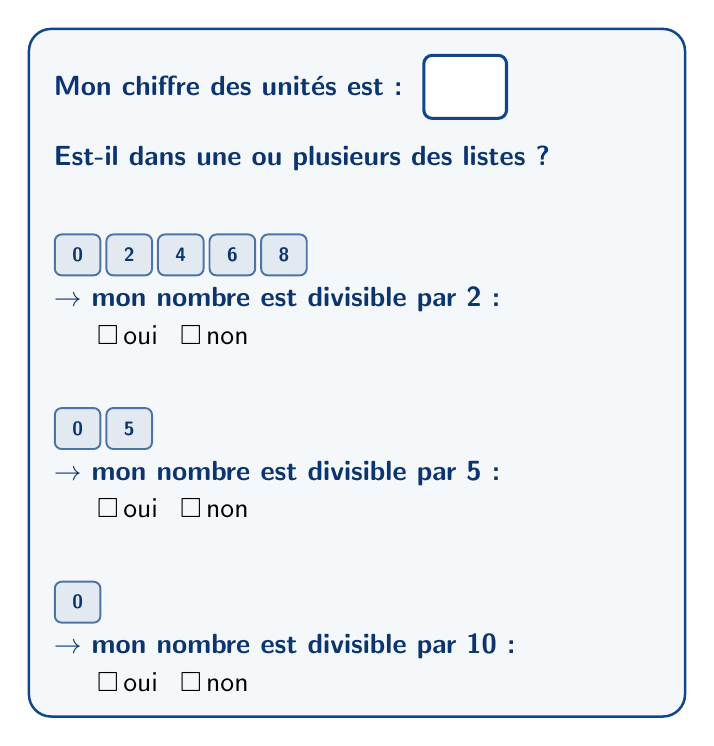
\begin{tikzpicture}
\node[rounded corners=8pt,draw=brandBlue,fill=brandBlue!4,line width=0.9pt,inner sep=9pt,align=left] {%
\begin{minipage}[t][8.10cm][s]{7.70cm}
{\bfseries\color{brandNavy} Mon chiffre des unités est :}\hspace{0.25cm}%
\tikz[baseline=-0.72ex]{\node[rounded corners=3pt,draw=brandBlue,fill=white,line width=1.1pt,minimum width=1.05cm,minimum height=0.80cm,font=\bfseries\fontsize{15}{15}\selectfont,text=penInk]{};}\par\vspace{0.30cm}
{\bfseries\color{brandNavy} Est-il dans une ou plusieurs des listes ?}\par\vfill
\Reglette{brandBlue}{0.58cm}{-1}{0,2,4,6,8}\par\vspace{0.12cm}
{\bfseries\color{brandNavy} $\rightarrow$ mon nombre est divisible par 2 :}\par\vspace{0.06cm}
\hspace*{0.55cm}\OuiNon{0}{0}\par\vfill
\Reglette{brandBlue}{0.58cm}{-1}{0,5}\par\vspace{0.12cm}
{\bfseries\color{brandNavy} $\rightarrow$ mon nombre est divisible par 5 :}\par\vspace{0.06cm}
\hspace*{0.55cm}\OuiNon{0}{0}\par\vfill
\Reglette{brandBlue}{0.58cm}{-1}{0}\par\vspace{0.12cm}
{\bfseries\color{brandNavy} $\rightarrow$ mon nombre est divisible par 10 :}\par\vspace{0.06cm}
\hspace*{0.55cm}\OuiNon{0}{0}%
\end{minipage}};
\end{tikzpicture}
\end{minipage}\hfill
% ---------------- Chemin B : somme des chiffres ----------------
\begin{minipage}[t]{10.75cm}
\StepHeadB{3}{Critères de divisibilité par 3 et 9}\par\vspace{0.10cm}
{\color{brandOrange}\fontsize{11.2}{12.2}\selectfont $\rightarrow$ J'\textbf{additionne} tous les chiffres}\par\vspace{0.14cm}
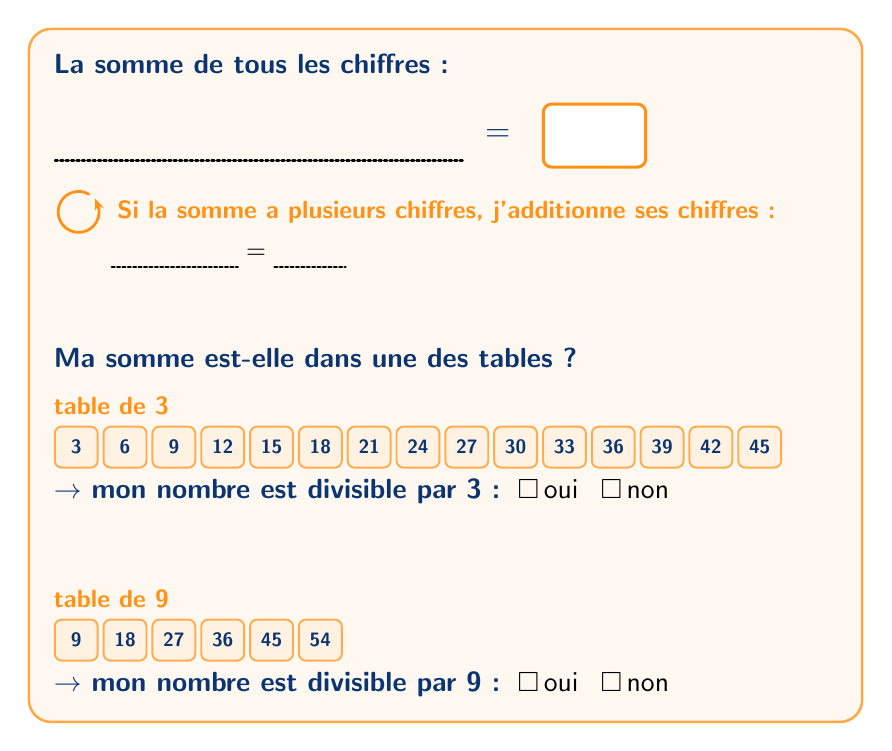
\begin{tikzpicture}
\node[rounded corners=8pt,draw=brandOrange!80,fill=brandOrange!6,line width=0.9pt,inner sep=9pt,align=left] {%
\begin{minipage}[t][8.10cm][s]{9.95cm}\raggedright
{\bfseries\color{brandNavy} La somme de tous les chiffres :}\par\vspace{0.34cm}
\LigneSomme{}{}\par\vspace{0.20cm}
{\small \BoucleFleche\hspace{0.18cm}{\bfseries\color{brandOrange} Si la somme a plusieurs chiffres, j'additionne ses chiffres :}}\par\vspace{0.08cm}
{\small \hspace{0.72cm}\LowDotted{1.60}\;$=$\;\LowDotted{0.90}}\par\vfill
{\bfseries\color{brandNavy} Ma somme est-elle dans une des tables ?}\par\vspace{0.18cm}
{\bfseries\small\color{brandOrange} table de 3}\par\vspace{0.10cm}
\Reglette{brandOrange}{0.545cm}{-1}{3,6,9,12,15,18,21,24,27,30,33,36,39,42,45}\par\vspace{0.12cm}
{\bfseries\color{brandNavy} $\rightarrow$ mon nombre est divisible par 3 :}\hspace{0.22cm}\OuiNon{0}{0}\par\vfill
{\bfseries\small\color{brandOrange} table de 9}\par\vspace{0.10cm}
\Reglette{brandOrange}{0.545cm}{-1}{9,18,27,36,45,54}\par\vspace{0.12cm}
{\bfseries\color{brandNavy} $\rightarrow$ mon nombre est divisible par 9 :}\hspace{0.22cm}\OuiNon{0}{0}%
\end{minipage}};
\end{tikzpicture}
\end{minipage}

\vspace{0.22cm}
\StepHead{4}{Je remplis mon tableau et je conclus}\par\vspace{0.16cm}
\begin{center}
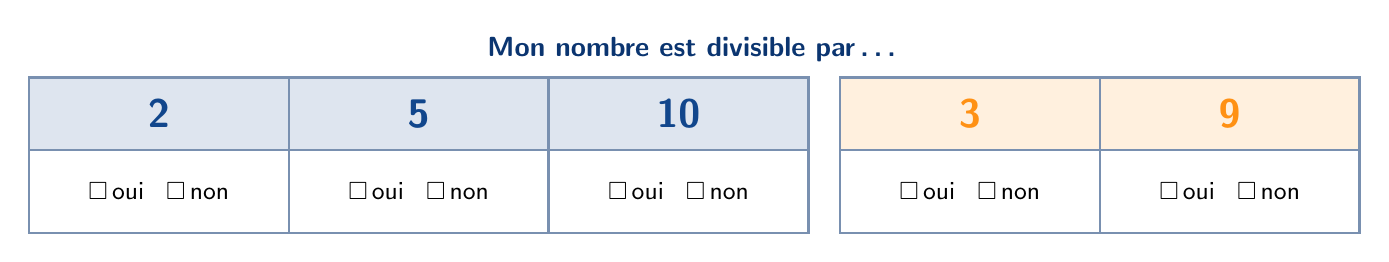
\begin{tikzpicture}[x=1cm,y=1cm]
  \def\colw{3.30}\def\rowa{0.92}\def\rowb{1.05}\def\ecart{0.40}
  \node[anchor=south,font=\bfseries\color{brandNavy}] at ({2.5*\colw+\ecart/2},{\rowa+\rowb+0.08}) {Mon nombre est divisible par\,\ldots};
  \foreach \i/\lab/\col in {0/2/brandBlue,1/5/brandBlue,2/10/brandBlue,3/3/brandOrange,4/9/brandOrange}{
    \pgfmathsetmacro{\xp}{\i*\colw + (\i>2 ? \ecart : 0)}
    \draw[fill=\col!14,draw=brandNavy!55,line width=0.85pt] (\xp,\rowb) rectangle +(\colw,\rowa);
    \node[font=\bfseries\fontsize{15}{15}\selectfont,text=\col] at ({\xp+\colw/2},{\rowb+\rowa/2}) {\lab};
    \draw[fill=white,draw=brandNavy!55,line width=0.85pt] (\xp,0) rectangle +(\colw,\rowb);
  }
  \foreach \i/\a/\b in {0/0/0,1/0/0,2/0/0,3/0/0,4/0/0}{
    \pgfmathsetmacro{\xp}{\i*\colw + (\i>2 ? \ecart : 0)}
    \node[font=\small] at ({\xp+\colw/2},{\rowb/2}) {\OuiNon{\a}{\b}};
  }
\end{tikzpicture}
\end{center}
\vspace{0.10cm}
\begin{center}
{\fontsize{9.8}{10.8}\selectfont\bfseries\color{brandNavy!80} Il y a peut-être d'autres diviseurs (4, 7, 11\ldots) : je le vérifie en posant une division.}
\end{center}

\vspace{0.12cm}
\begin{center}
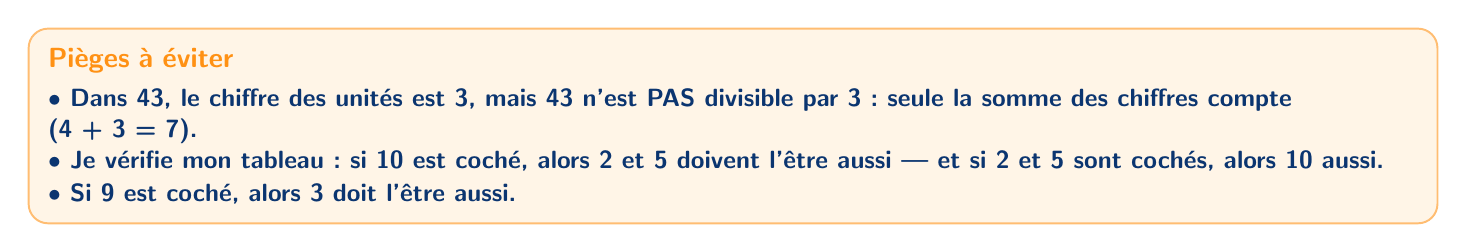
\begin{tikzpicture}
\node[rounded corners=7pt,draw=brandOrange!60,fill=softOrange!60,line width=0.7pt,text width=17.4cm,inner sep=7pt,align=left] {
{\bfseries\color{brandOrange} Pièges à éviter}\par\vspace{0.10cm}
{\fontsize{9.3}{11.2}\selectfont\bfseries\color{brandNavy} $\bullet$ Dans 43, le chiffre des unités est 3, mais 43 n'est PAS divisible par 3 : seule la somme des chiffres compte \mbox{(4 + 3 = 7)}.\par
$\bullet$ Je vérifie mon tableau : si 10 est coché, alors 2 et 5 doivent l'être aussi — et si 2 et 5 sont cochés, alors 10 aussi.\par
$\bullet$ Si 9 est coché, alors 3 doit l'être aussi.}
};
\end{tikzpicture}
\end{center}

\newpage

% =====================================================================
% PAGE 2 : VERSO — le meme outil, entierement redige (exemple : 8 595)
% =====================================================================
\EnTete{\tikz{\node[rounded corners=6pt,draw=penInk!60,fill=white,line width=0.8pt,inner xsep=9pt,inner ysep=5pt,font=\bfseries\fontsize{10.6}{11.4}\selectfont,text=penInk]{Exemple entièrement rédigé : je teste 8\,595};}}

\StepHead{1}{J'écris mon nombre}\par\vspace{0.30cm}
\begin{center}
\CasesNombre{}{}{8}{5}{9}{5}{1}
\end{center}
\vspace{0.18cm}

\noindent
\begin{minipage}[t]{8.45cm}
\StepHeadB{2}{Critères de divisibilité par 2, 5 et 10}\par\vspace{0.10cm}
{\color{brandBlue}\fontsize{11.2}{12.2}\selectfont $\rightarrow$ Je \textbf{regarde} le chiffre des unités}\par\vspace{0.14cm}
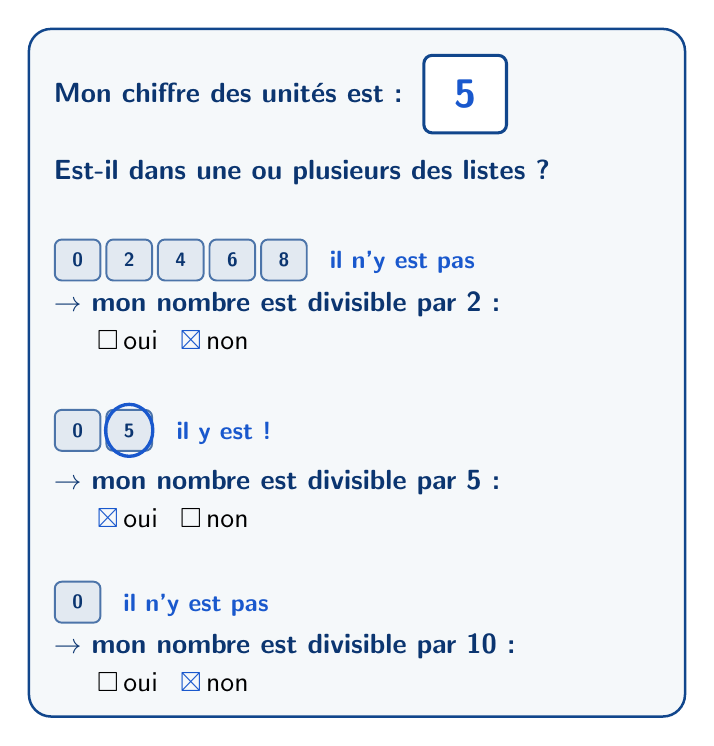
\begin{tikzpicture}
\node[rounded corners=8pt,draw=brandBlue,fill=brandBlue!4,line width=0.9pt,inner sep=9pt,align=left] {%
\begin{minipage}[t][8.10cm][s]{7.70cm}
{\bfseries\color{brandNavy} Mon chiffre des unités est :}\hspace{0.25cm}%
\tikz[baseline=-0.72ex]{\node[rounded corners=3pt,draw=brandBlue,fill=white,line width=1.1pt,minimum width=1.05cm,minimum height=0.80cm,font=\bfseries\fontsize{15}{15}\selectfont,text=penInk]{5};}\par\vspace{0.30cm}
{\bfseries\color{brandNavy} Est-il dans une ou plusieurs des listes ?}\par\vfill
\Reglette{brandBlue}{0.58cm}{-1}{0,2,4,6,8}\hspace{0.28cm}\Pen{\small il n'y est pas}\par\vspace{0.12cm}
{\bfseries\color{brandNavy} $\rightarrow$ mon nombre est divisible par 2 :}\par\vspace{0.06cm}
\hspace*{0.55cm}\OuiNon{0}{1}\par\vfill
\Reglette{brandBlue}{0.58cm}{5}{0,5}\hspace{0.28cm}\Pen{\small il y est !}\par\vspace{0.12cm}
{\bfseries\color{brandNavy} $\rightarrow$ mon nombre est divisible par 5 :}\par\vspace{0.06cm}
\hspace*{0.55cm}\OuiNon{1}{0}\par\vfill
\Reglette{brandBlue}{0.58cm}{-1}{0}\hspace{0.28cm}\Pen{\small il n'y est pas}\par\vspace{0.12cm}
{\bfseries\color{brandNavy} $\rightarrow$ mon nombre est divisible par 10 :}\par\vspace{0.06cm}
\hspace*{0.55cm}\OuiNon{0}{1}%
\end{minipage}};
\end{tikzpicture}
\end{minipage}\hfill
\begin{minipage}[t]{10.75cm}
\StepHeadB{3}{Critères de divisibilité par 3 et 9}\par\vspace{0.10cm}
{\color{brandOrange}\fontsize{11.2}{12.2}\selectfont $\rightarrow$ J'\textbf{additionne} tous les chiffres}\par\vspace{0.14cm}
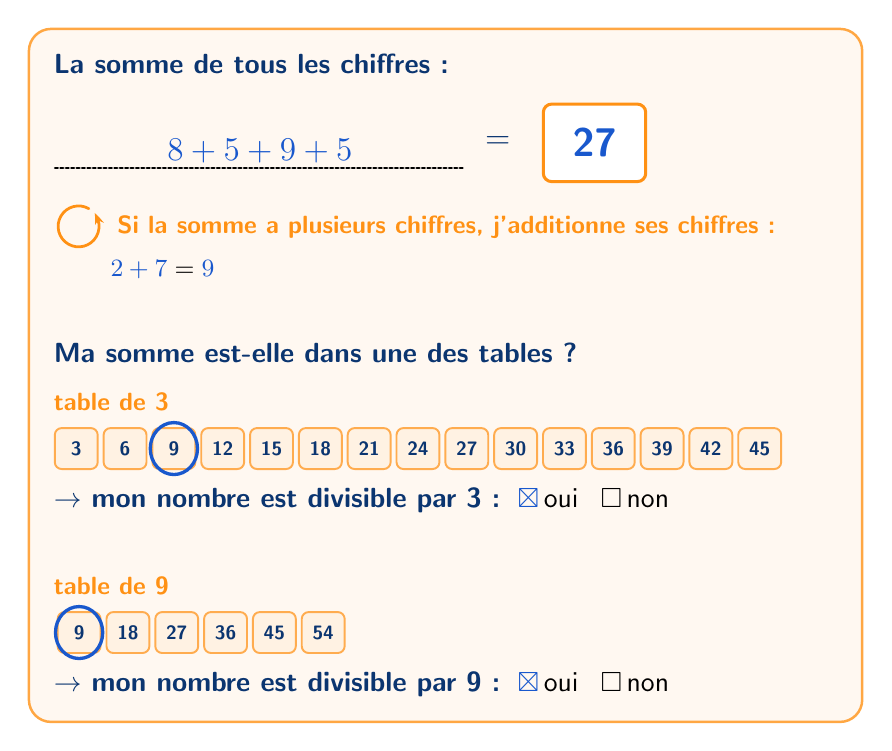
\begin{tikzpicture}
\node[rounded corners=8pt,draw=brandOrange!80,fill=brandOrange!6,line width=0.9pt,inner sep=9pt,align=left] {%
\begin{minipage}[t][8.10cm][s]{9.95cm}\raggedright
{\bfseries\color{brandNavy} La somme de tous les chiffres :}\par\vspace{0.34cm}
\LigneSomme{\Pen{$8+5+9+5$}}{27}\par\vspace{0.20cm}
{\small \BoucleFleche\hspace{0.18cm}{\bfseries\color{brandOrange} Si la somme a plusieurs chiffres, j'additionne ses chiffres :}}\par\vspace{0.08cm}
{\small \hspace{0.72cm}\Pen{$2+7$}\;$=$\;\Pen{$9$}}\par\vfill
{\bfseries\color{brandNavy} Ma somme est-elle dans une des tables ?}\par\vspace{0.18cm}
{\bfseries\small\color{brandOrange} table de 3}\par\vspace{0.10cm}
\Reglette{brandOrange}{0.545cm}{9}{3,6,9,12,15,18,21,24,27,30,33,36,39,42,45}\par\vspace{0.12cm}
{\bfseries\color{brandNavy} $\rightarrow$ mon nombre est divisible par 3 :}\hspace{0.22cm}\OuiNon{1}{0}\par\vfill
{\bfseries\small\color{brandOrange} table de 9}\par\vspace{0.10cm}
\Reglette{brandOrange}{0.545cm}{9}{9,18,27,36,45,54}\par\vspace{0.12cm}
{\bfseries\color{brandNavy} $\rightarrow$ mon nombre est divisible par 9 :}\hspace{0.22cm}\OuiNon{1}{0}%
\end{minipage}};
\end{tikzpicture}
\end{minipage}

\vspace{0.22cm}
\StepHead{4}{Je remplis mon tableau et je conclus}\par\vspace{0.16cm}
\begin{center}
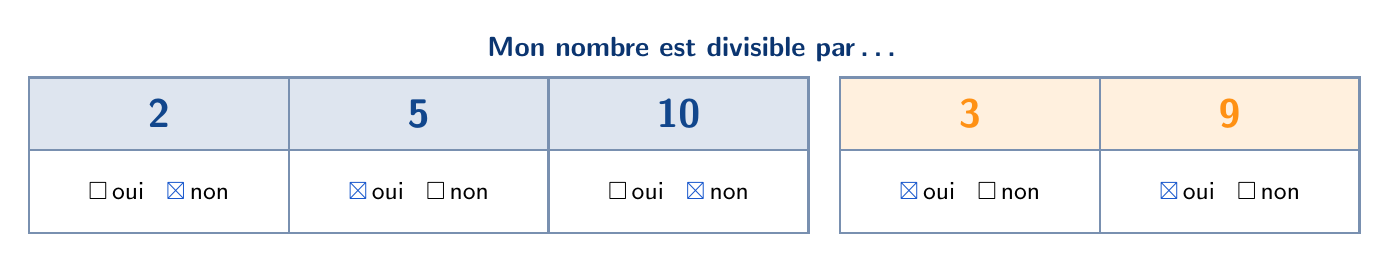
\begin{tikzpicture}[x=1cm,y=1cm]
  \def\colw{3.30}\def\rowa{0.92}\def\rowb{1.05}\def\ecart{0.40}
  \node[anchor=south,font=\bfseries\color{brandNavy}] at ({2.5*\colw+\ecart/2},{\rowa+\rowb+0.08}) {Mon nombre est divisible par\,\ldots};
  \foreach \i/\lab/\col in {0/2/brandBlue,1/5/brandBlue,2/10/brandBlue,3/3/brandOrange,4/9/brandOrange}{
    \pgfmathsetmacro{\xp}{\i*\colw + (\i>2 ? \ecart : 0)}
    \draw[fill=\col!14,draw=brandNavy!55,line width=0.85pt] (\xp,\rowb) rectangle +(\colw,\rowa);
    \node[font=\bfseries\fontsize{15}{15}\selectfont,text=\col] at ({\xp+\colw/2},{\rowb+\rowa/2}) {\lab};
    \draw[fill=white,draw=brandNavy!55,line width=0.85pt] (\xp,0) rectangle +(\colw,\rowb);
  }
  \foreach \i/\a/\b in {0/0/1,1/1/0,2/0/1,3/1/0,4/1/0}{
    \pgfmathsetmacro{\xp}{\i*\colw + (\i>2 ? \ecart : 0)}
    \node[font=\small] at ({\xp+\colw/2},{\rowb/2}) {\OuiNon{\a}{\b}};
  }
\end{tikzpicture}
\end{center}
\vspace{0.10cm}
\begin{center}
{\fontsize{9.8}{10.8}\selectfont\bfseries\color{brandNavy!80} Il y a peut-être d'autres diviseurs (4, 7, 11\ldots) : je le vérifie en posant une division.}
\end{center}

\vspace{0.12cm}
\begin{center}
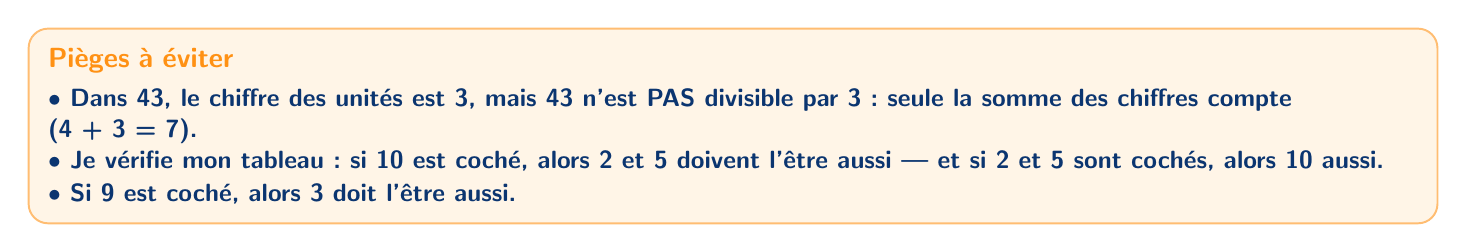
\begin{tikzpicture}
\node[rounded corners=7pt,draw=brandOrange!60,fill=softOrange!60,line width=0.7pt,text width=17.4cm,inner sep=7pt,align=left] {
{\bfseries\color{brandOrange} Pièges à éviter}\par\vspace{0.10cm}
{\fontsize{9.3}{11.2}\selectfont\bfseries\color{brandNavy} $\bullet$ Dans 43, le chiffre des unités est 3, mais 43 n'est PAS divisible par 3 : seule la somme des chiffres compte \mbox{(4 + 3 = 7)}.\par
$\bullet$ Je vérifie mon tableau : si 10 est coché, alors 2 et 5 doivent l'être aussi — et si 2 et 5 sont cochés, alors 10 aussi.\par
$\bullet$ Si 9 est coché, alors 3 doit l'être aussi.}
};
\end{tikzpicture}
\end{center}

\end{document}
